\maketitle
\section*{The Universe}
In the beginning the Universe was created. This has made a lot of people very angry and been widely regarded as a bad move.
I know why everybody is this angry about it, but it really just sounds like their problem.

In figure \ref{fig:universe} you can see a picture of a galaxy.

\begin{figure}[h]
  \center
  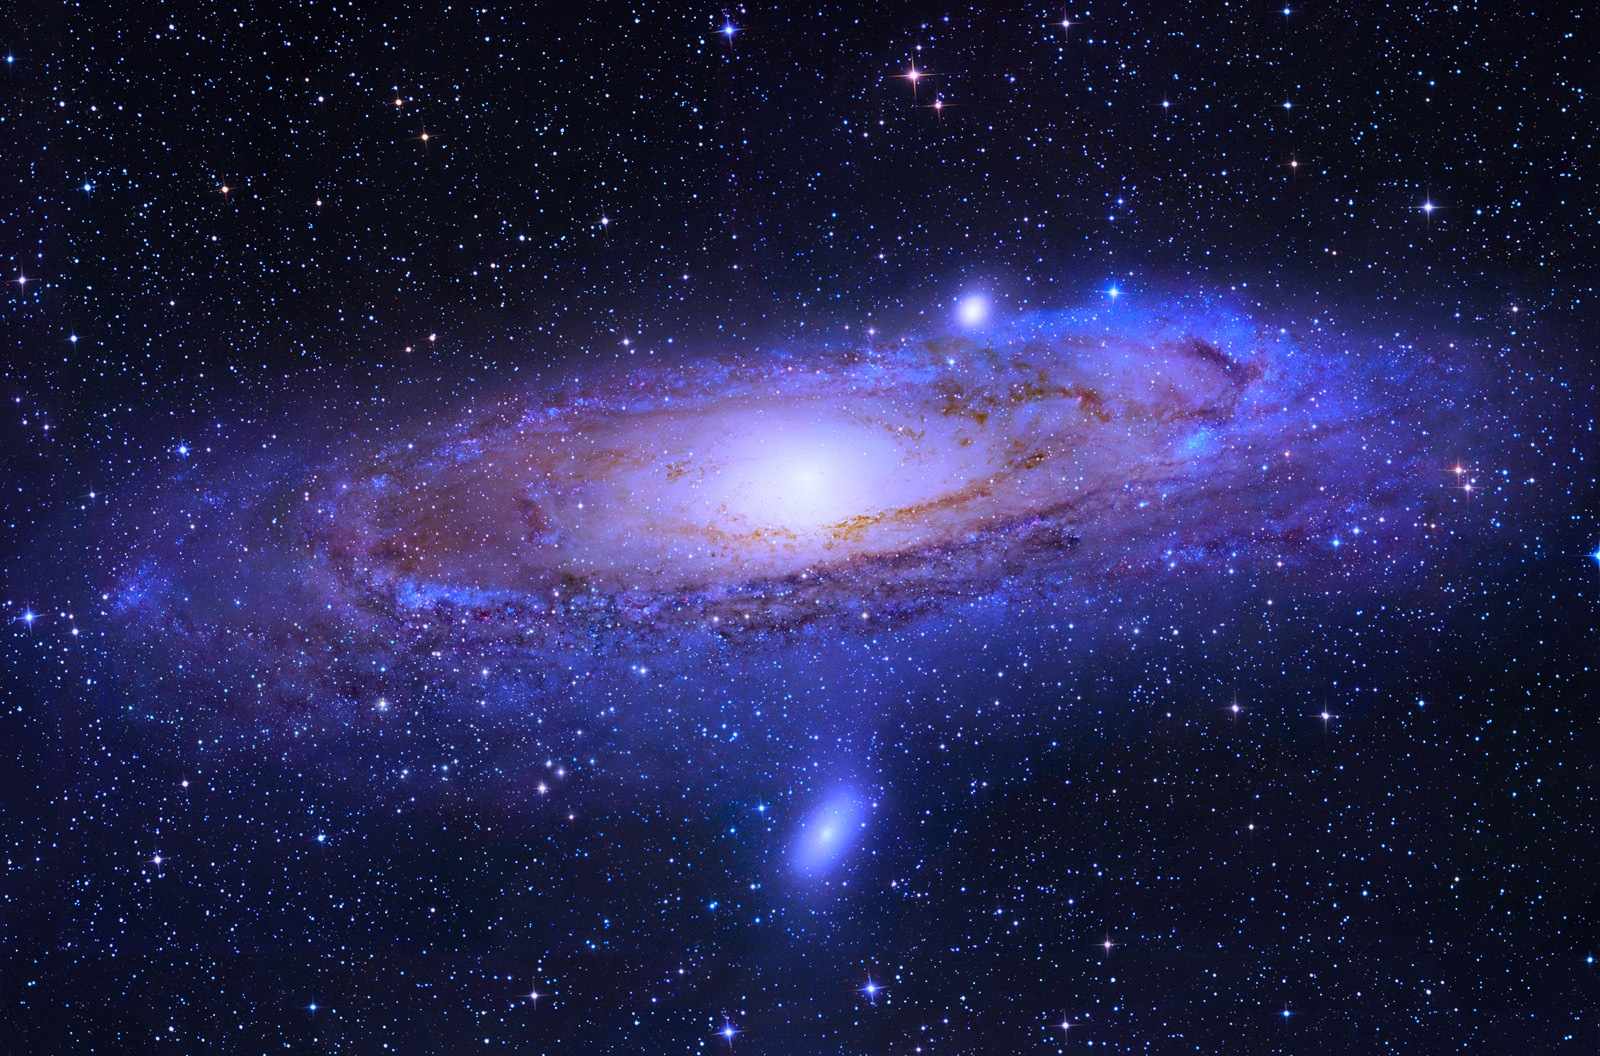
\includegraphics[width=0.6\textwidth]{galaxy.jpg}
  \caption{A picture of a galaxy}
  \label{fig:universe}
\end{figure}

A galaxy is really big. You're just a tiny spec of dust in comparison. Now, there are a lot of galaxies in the universe.
So many indeed, that there are galaxy clusters, where multiple galaxies are grouped together based on the distance between them.
But that's not enough yet. There are also clusters of clusters. And then there's groups of clusters.

The universe is really big. We don't even really know how big. Why? We can't even see it's borders, because light from there hasn't reached us yet.

In a believed stroke of genius, some may say that there's still something more massive, your mom. However, since we're here to proof that you're insignificant,
your mom can't be this massive, or it would be something you'd be significant for.

\section{The Beginning}

Now let's talk about how everything came to be. Since, you know, I'm God, I have utmost authority when speaking about how things came to be.

Now, in another believed stroke of genius, some may say that everything came to be, because I fucked your mom. However, I'm God, so I have higher standards.

What actually happened, is that I just felt like torturing some innocent souls of the aether for existing, so I just made an endless place of torment to place them into.
This has backfired immensly though, because somehow, somewhy, some people believe that there's a way to salvation and that I love them and so on. I don't realy know how the fuck
you'd think that, but you do you. Now I could end this paper here and have you conclude on your own that you're insignificant, because I obviously created you to torture you, but
I feel like shitting on you some more, so this is only \emph{the Beginning}.

\begin{center}
  Have fun!
\end{center}
\section{Your Beginning}

It doesn't matter.
\section{Your Life}

Holy fuck, how did you even get this far? Your life has no meaning, you have no reason to exist. Why didn't you kill yourself already?
Well, since you're here anyways, I can prove to you how you existing does not add anything to the universe at all.
Let $a : \text{People} \rightarrow \mathbb{N}$, with 
$$a(x) = \text{number of meaningful achievemnts of } x$$
where $x \in \text{People}$.

Now you might think that on a bell curve of intelligence, like the one shown in 
figure \ref{fig:bell-curve}, the graph plotting the average of 
$$a(x_1), a(x_2), \dotsc, a(x_{n-1}), a(x_n)$$
with $x_i \in \{x \in \text{People } | \text{ IQ of } x \text{ is the current IQ}\}$ over the IQ, would resemble an exponential one, because
you'd think that the more intelligent someone was, the more they would achieve in their life. I would wager that the vast amount of people
think like this. However, it isn't true.

\begin{figure}[h]
  \center
  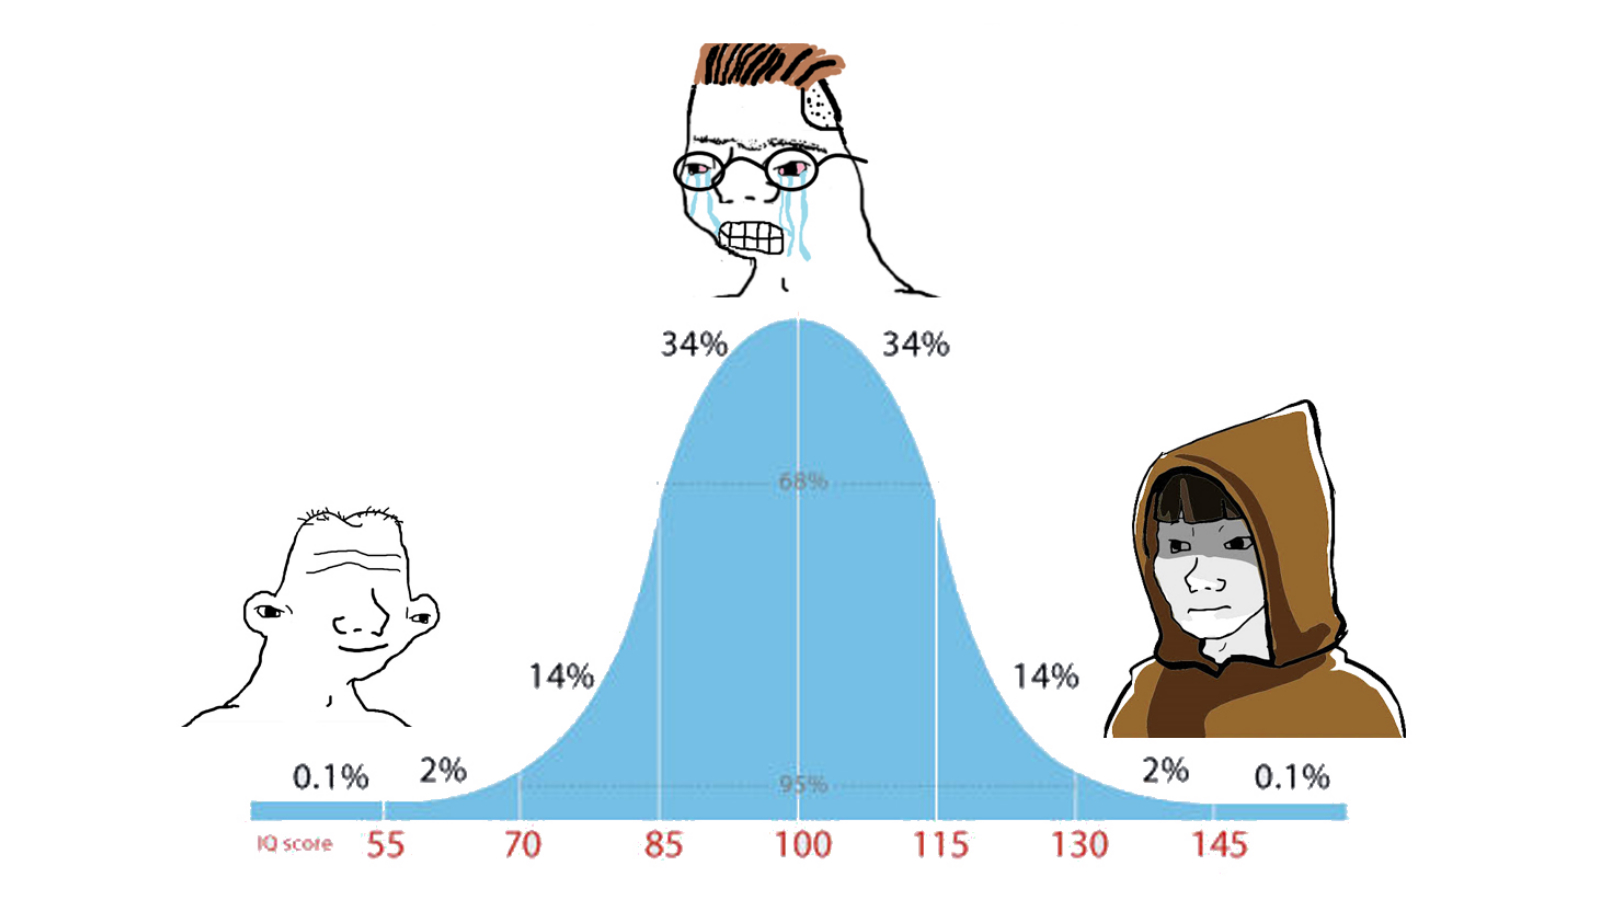
\includegraphics[width=0.8\textwidth]{bell-curve.jpg}
  \caption{The intelligence bell curve}
  \label{fig:bell-curve}
\end{figure}

Another thing you might think is that it could also behave like the bell curve itself. The reasoning behind it might be the conclusion that
once you become too intelligent, you overthink a lot and it prevents you from actually getting things done.

However, I'm here to tell you that it would probably rather look something like the graph shown in figure \ref{fig:graph-achievements}.
Why do I say that? Well, because no human being has ever achieved something meaningful. Nothing you or anybody else has ever done has
contributed something to the universe. And I'm certain of that, because I made it that way.

\begin{figure}[h]
  \center
  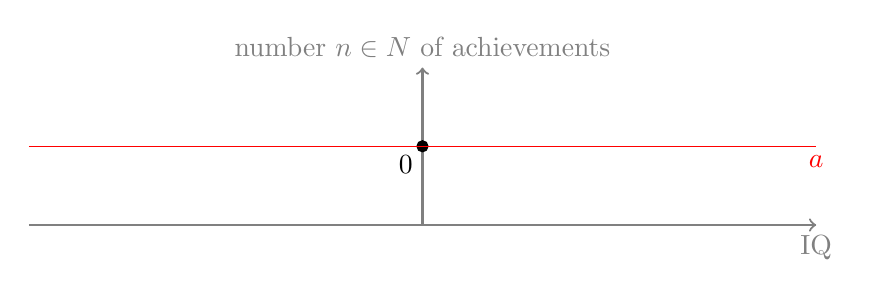
\begin{tikzpicture}
    \draw[->, gray, thick] (-5, -1) -- (5, -1) node[anchor=north]{IQ};
    \draw[->, gray, thick] (0, -1) -- (0, 1) node[anchor=south]{number $n \in \mathbb{N}$ of achievements};
    \filldraw[black] (0,0) circle (2pt) node[anchor=north east]{0};
    \draw[red, thin] (-5, 0) -- (5, 0) node[anchor=north]{$a$};
  \end{tikzpicture}
  \caption{Average amount of meaningful achievements per step of IQ}
  \label{fig:graph-achievements}
\end{figure}

\section{Significance}

So, you haven't achieved anything meaningful. That doesn't have to mean that you're insignificant. Maybe you're significant, because you have
a weird name, like "X Æ A-12", or you're the father of someone called "X Æ A-12". People know you, so you're significant, but you haven't achieved
anything.

\vspace{.5cm}

So, what does it mean to be significant? Does it mean that people know you? Does it mean that you achieved something meaningful?
Does it mean that you dying would be a bad thing? Does it mean that I care about you?

Well, everything except for that last part. I don't give a shit about any of you. Now let's define significance in a more formal manner.
Let's use first order logic to codify humanity. We will start with $\Sigma$ and what the constants mean.

$$
\begin{aligned}
  \Sigma &= \left( \right\{ \nicefrac{a}{0}, \nicefrac{e}{0} \left\}, \left\{ \nicefrac{P}{1}, \nicefrac{K}{1}, \nicefrac{A}{1}, \nicefrac{D}{1}, \nicefrac{C}{3} \right\} \right) \\
  a &:= \text{"Adam"}, \\
  e &:= \text{"Eve"}
\end{aligned}
$$
After this definition we have the constants $a$ and $e$, representing Adam and Eve respectively.
Now, let's define the predicates:

$$
\begin{aligned}
  P(x) &:= \text{"} x \text{ is a person"}\\
  K(x) &:= \text{"} x \text{ is known"}\\
  A(x) &:= \text{"} x \text{ has achieved something meaningful"}\\
  D(x) &:= \text{"} x \text{ dying would be a bad thing"}\\
  C(x, y, z) &:= \text{"} x \text{ is child of } y \text{ and } z \text{"}
\end{aligned}
$$

Now what does all this tell us so far? Well, we know that there are people. We also know that there are
the constants $a$ and $e$, which, at least in this model, aren't considered people. We also know that $x$
could be known ($K(x)$), $x$ could have achieved something meaningful ($A(x)$) and that $x$ dying could be
a bad thing ($D(x)$). We also know that $x$ could be a child of $y$ and $z$ ($C(x, y, z)$).
We can now already formulate some things about people. Let's do so.
Here's the formula for significance:

$$
\text{isSignificant}(x) ::= P(x) \wedge \left(K(x) \vee A(x) \vee D(x)\right)
$$
And now, let's codify some of humanity:

$$
\begin{aligned}
  \forall x &. P(x) \rightarrow \left(\exists y,z . C(x, y, z)\right) \vee C(x, a, e)\\
  \exists x &. \text{isSignificant}(x)
\end{aligned}
$$

At this point, we know that each person $x$ has a pair of parents. These could be other people, or the parents of $x$
could be $a$ and $e$. We have also defined what it means to be significant. In our case it means that the formula $\text{isSignificant}(x)$
is true for the given $x$. We have also said that there exists at least one person, who is significant.